%! Author = samrelins
%! Date = 08/06/2022

\subsection{Design}

This was a retrospective data linkage study. Our aim was to replicate the work of Wright et al., demonstrating the link between EYFSP scores and ASD and, in general, the utility of large connected datasets. This study expands the cohort beyond participants in the Born in Bradford study, to the entire Bradford district using Connected Bradford data. Connected Bradford hosts post-2013 EYFSP scores and education census data up to the 2019 academic year, comprising the 70,277 unique individuals assessed for the EYFSP in the Bradford district during that period, inclusive of the 8,935 children from the Wright study. Education data were linked with primary care records collected from 86 GP surgeries in the Bradford district.

\subsection{EYFSP Observations}

 The Early Year's Foundation Stage Profile - EYFSP - summarises and describes children's learning and development in accordance with 7 areas of learning, subdivided into 17 early learning goals (Figure \ref{fig:eyfsp_info}). Assessments are conducted in the final term of the year in which a child reaches age 5 and are used to support the transition into the national curriculum Key Stage 1. Scoring is based on an observational assessment conducted by teaching practitioners and guided by a framework set out by the UK Department for Education\cite{eyfsp_handbook}. Scores are recorded for each goal as ``emerging'' (not meeting the expected level of development for this goal), ``expected'' (meeting the expected level of development), ``exceeding'' (exceeding the expected level of development), or ``absent for long periods or recently arrived''. For the purposes of this study the ``absent for long periods or recently arrived'' is considered a missing or NA result.

\begin{table}[h]
    \centering
    \begin{scriptsize}\begin{tabular}{P{68mm}P{62mm}}
        \toprule
         &  \\
        \textbf{Communication and language development} & \textbullet Listening and attention \\
         & \textbullet Understanding \\
         & \textbullet Speaking \\[3mm]
        \textbf{Physical development} & \textbullet Moving and handling \\
         & \textbullet Health and self-care \\[3mm]
        \textbf{Personal, social and emotional development} & \textbullet Self-confidence and self-awareness \\
         & \textbullet Managing feelings and behaviour \\
         & \textbullet Making relationships \\[3mm]
        \textbf{Literacy} & \textbullet Reading \\
         & \textbullet Writing \\[3mm]
        \textbf{Mathematics} & \textbullet Numbers \\
         & \textbullet Shape, space and measures \\[3mm]
        \textbf{Understanding of the world} & \textbullet People and communities \\
         & \textbullet The world \\
         & \textbullet Technology \\[3mm]
        \textbf{Expressive arts and design} & \textbullet Exploring and using media and materials \\
         & \textbullet Being imaginative \\[3mm]
        \bottomrule
    \end{tabular}\end{scriptsize}
    \captionof{figure}{The 17 early learning goals as defined in the Early Years Foundation Stage profile}
    \label{fig:eyfsp_info}
\end{table}

As with the Wright et al. methodology, we used only post-2013 EYFSP results and aggregated the results according to the following method: goals assessed as emerging were scored 1, expected were scored 2 and exceeding 3. Total scores were calculated for each individual, as well as the same 5-item subscore used by Wright et al. developed by a group of ASD assement experts (Figure \ref{fig:subscore_info}).

\begin{table}[h]
    \centering
    \begin{scriptsize}\begin{tabular}{P{35mm}P{90mm}}
                          \toprule
                          \multicolumn{2}{P{125mm}}{\textbf{EYFSP Weighted Subscore:}} \\[2mm]
                          \multicolumn{2}{P{125mm}}{Using a weighted subscore, where four aspects of childhood autism (social, language and communications, imagination and repetitive behaviour) were mapped onto EYFSP elements} \\[5mm]
                          \textbf{Speaking} & \textbullet Personal, social and emotional: managing feelings and behaviour  \\
                           & \textbullet Personal, social and emotional: making relationships \\[2mm]
                          \textbf{Social} & \textbullet Communication and language: listening and attention \\[2mm]
                          \textbf{Imagination} & \textbullet Expressive arts and design: being imaginative \\[2mm]
                          \textbf{Repetitive Behaviour} & \textbullet Physical development: health and self-care\\[2mm]
                          \bottomrule
    \end{tabular}\end{scriptsize}
    \captionof{figure}{Five item EYFSP subscore. The five learning goals used in the subscore were chosen from the four main syptom areas defined in the WHO (1992) research diagnostic criteria for ASD - social reciprocity, language and communication, imagination delays and repetitive and stereotyped patterns of behaviour. Because the social reciprocity domain is given more weight in this classification system, it was decided to include two items from the EYFSP to reflect this weighting}
    \label{fig:subscore_info}
\end{table}
\subsection{SNOMED coding of ASD}

Unlike the "read codes" used in the primary care records in Born in Bradford, the Connected Bradford data use the more up-to-date SNOMED-CT codings currently in use by GP practices. As such, we compiled a list of relevant SNOMED codes to identify autism spectrum disorders.

SNOMED-CT is a heirachical coding system. Conditions are organised in a tree-like structure with ``parent'' conditions and decendant ``child'' conditions. The ``children'' are considered to be more specific sub-divisions of the ``parent'' conditions from which they descend. For example, a patient may be diagnosed with ``Epilepsy, SCTID: 84757009'', whilst another patient may be diagnosed with the more specific child condition ``Acquired epileptic aphasia, SCTID: 230438007'' - the second patient could also be considered to have ``Epilepsy'', as it is a ``parent'' of the condition they've been diagnosed with.

We identified ASD in the SNOMED-CT codings as ``Pervasive Developmental Disorder, SCTID: 35919005'' (``Autism Spectrum Disorders'' are listed as a secondary preferred term under this code). We then proceeded to collect 49 descendant conditions of this code, and used this list as our indicator of an ASD diagnosis[REFERENCE TO SNOMEDS TABLE - PROBS IN APPENDIX]. This method identified 1227 individuals, 1.75\% of our cohort, as having an ASD diagnosis; this proportion is in line with expected population levels.

\subsection{Analysis}

Following the same methodology as Wright et al. we used logistic regression to model the association between EYFSP scores and ASD diagnoses, using the python Statsmodels package\cite{statsmodels}. We included the same covariates: sex (male/female), free school meal status, ethnicity (grouped into White British/Pakistani/other ethnicity) and age of child at date of extract. We also chose to add an interaction term between sex and EYFSP score, as we hypothesized that sex and EYFSP performance are likely not independent of one another.
EYFSP scores ranged from a total of 17 to 51, with mean 32.87 and SD 8.01, and a 5-item subscore of 5 to 15, mean 9.94 and SD 2.40. As in the previous study, the scores show a bimodal distribution with a distinct group of children achieving the expected level of development and another somewhat distinct group with a majority of ``emerging'' development levels (Figure \ref{fig:density_plots}). As such, we chose to use the same approach to dichotomising the EYFSP scores, defining an individual score as "low" or "not low" according to a cutoff \textless  1 SD below the mean - this was a total score of less than 25 and a 5-item subscore of less than 8.

\begin{figure}[h]
    \centering
    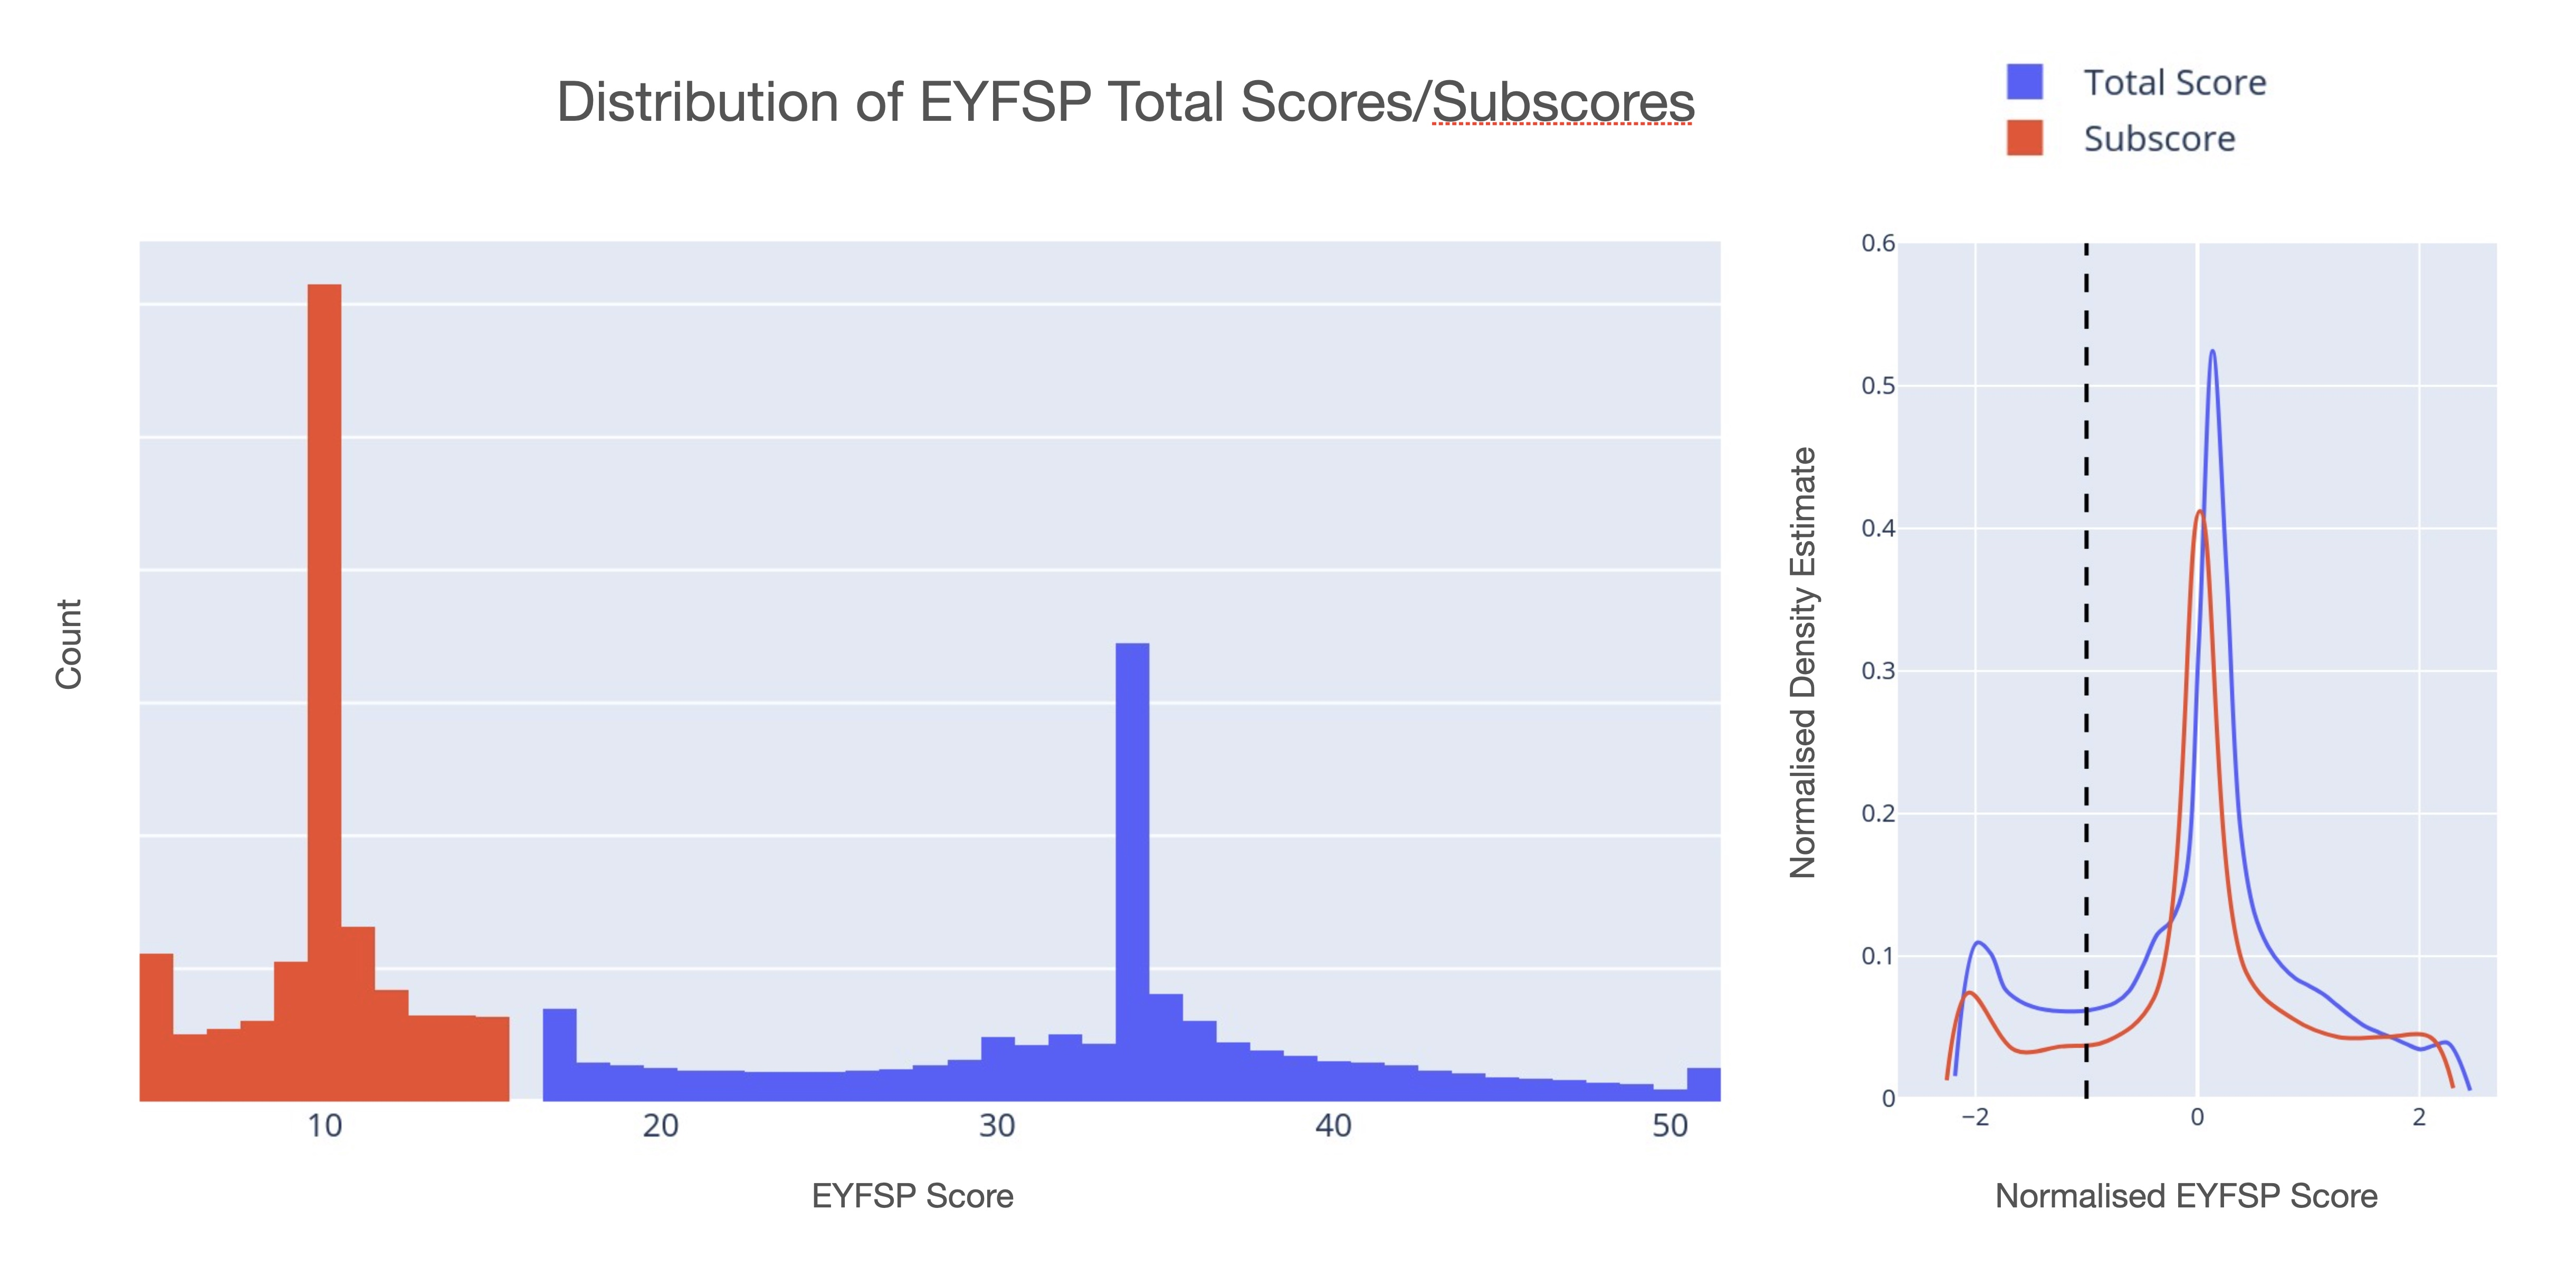
\includegraphics[width=1\textwidth]{density_plots}
    \caption{Histogram of EYFSP total and sub-scores (left) and normalised Kernel Density Estimates for distribution of Total Scores/Subscores (right). The black dashed line on the right plot represents the \textless1 SD boundary for defining ``low'' scores/subscores}
    \label{fig:density_plots}
\end{figure}

\newpage

